\section{Architecting TLBs in DRAM } 
\label{sec:stackedTLB}

\noindent When the application working set exceeds the TLB coverage
provided by UCAT (e.g., in $GUPS$), UCAT does not reduce the number of
memory accesses on an LLT miss. Reducing the number of memory accesses
on an LLT miss reduces effective LLT miss latency and also improves 
system memory access bandwidth.

We propose to increase TLB coverage by extending the TLB hierarchy
using {\em TLBs in DRAM (DRAM-TLB)}. DRAM-TLB logically sits between
the on-die shared LLT (or UCAT) and the page tables in memory.
DRAM-TLB is first consulted on an LLT (or UCAT) miss before walking
the page table (see Figure~\ref{fig:stacked_tlb}).

% \noindent Recent proposals extend the processor cache hierarchy by
% architecting stacked memory as a high capacity hardware-managed DRAM
% cache~\cite{BEAR, moin2012, unison, loh2011, jaewoong2012}. Similarly,

\begin{figure*}[t] 
  \vspace{-0. in} \centering
%  \centerline{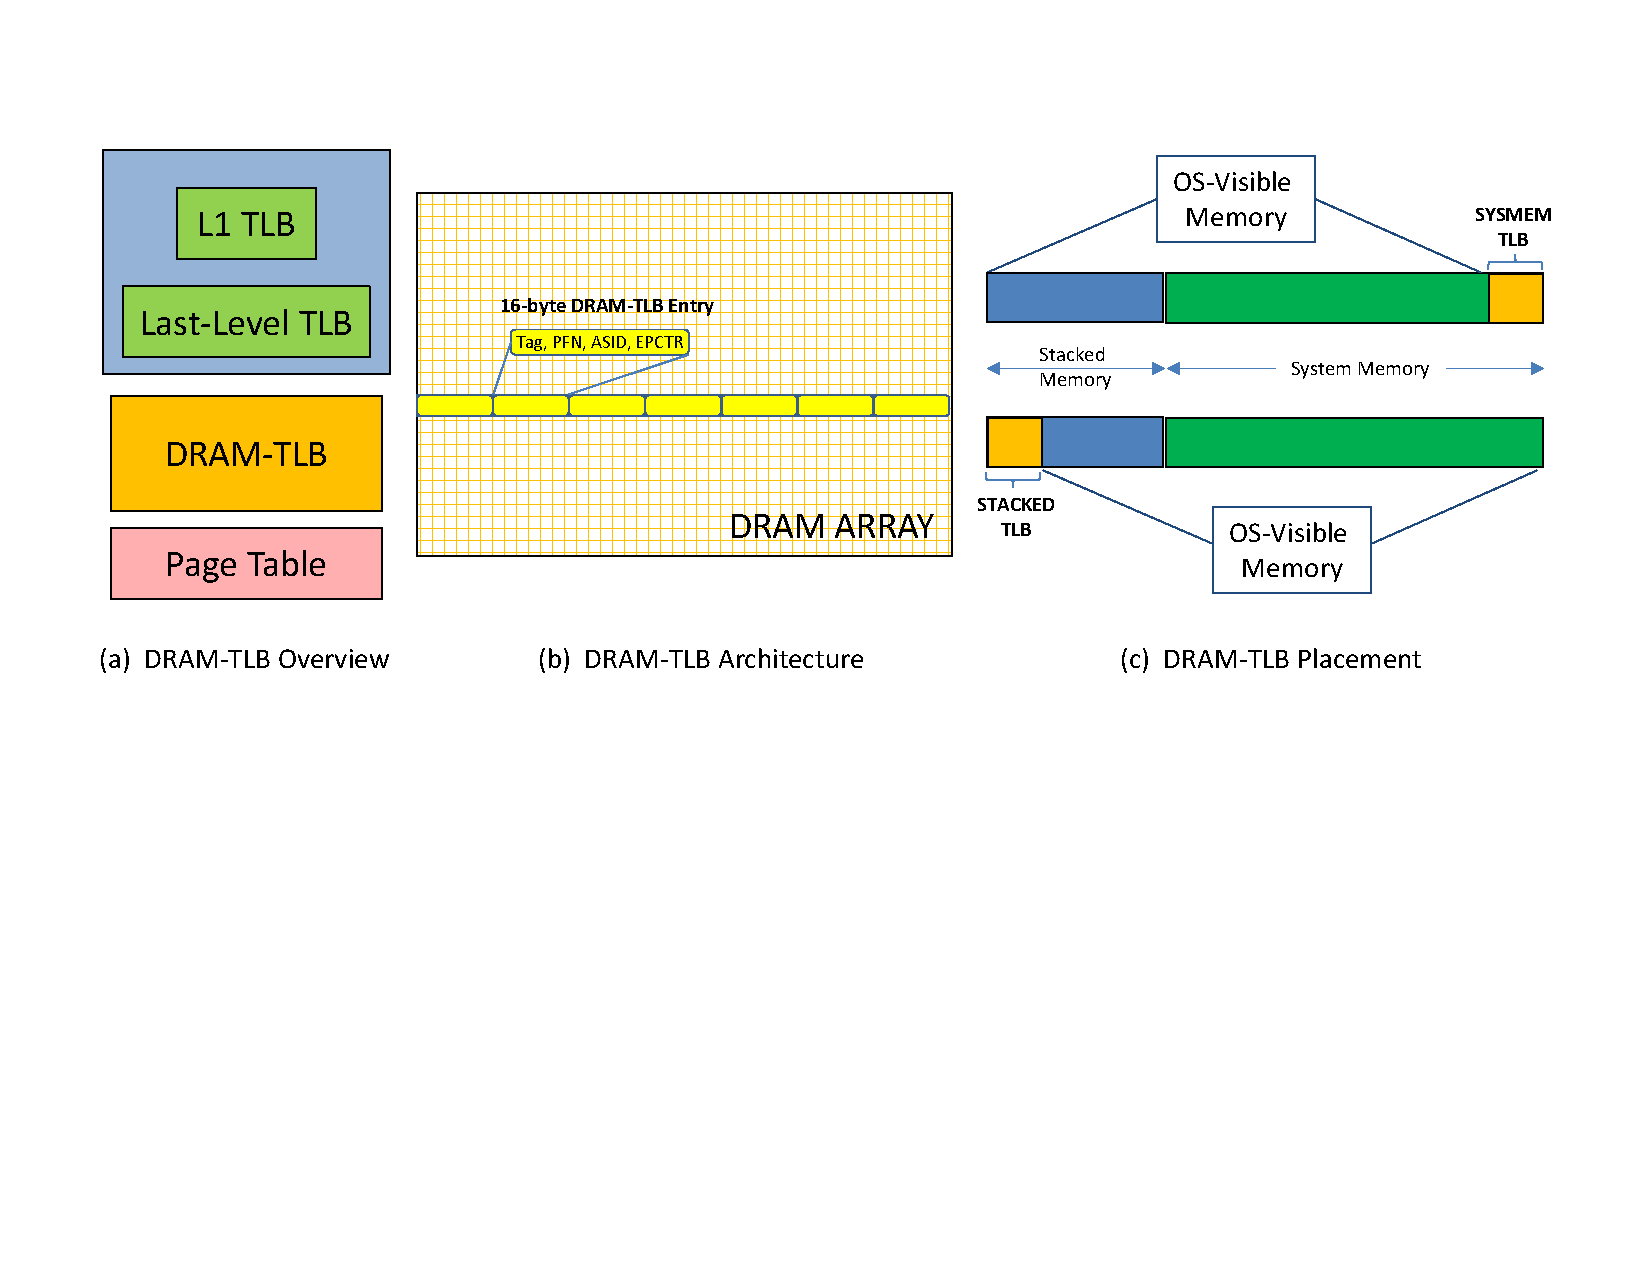
\psfig{file=FIGURES/stacked_tlb,angle=-90,width=\columnwidth}}
   \centerline{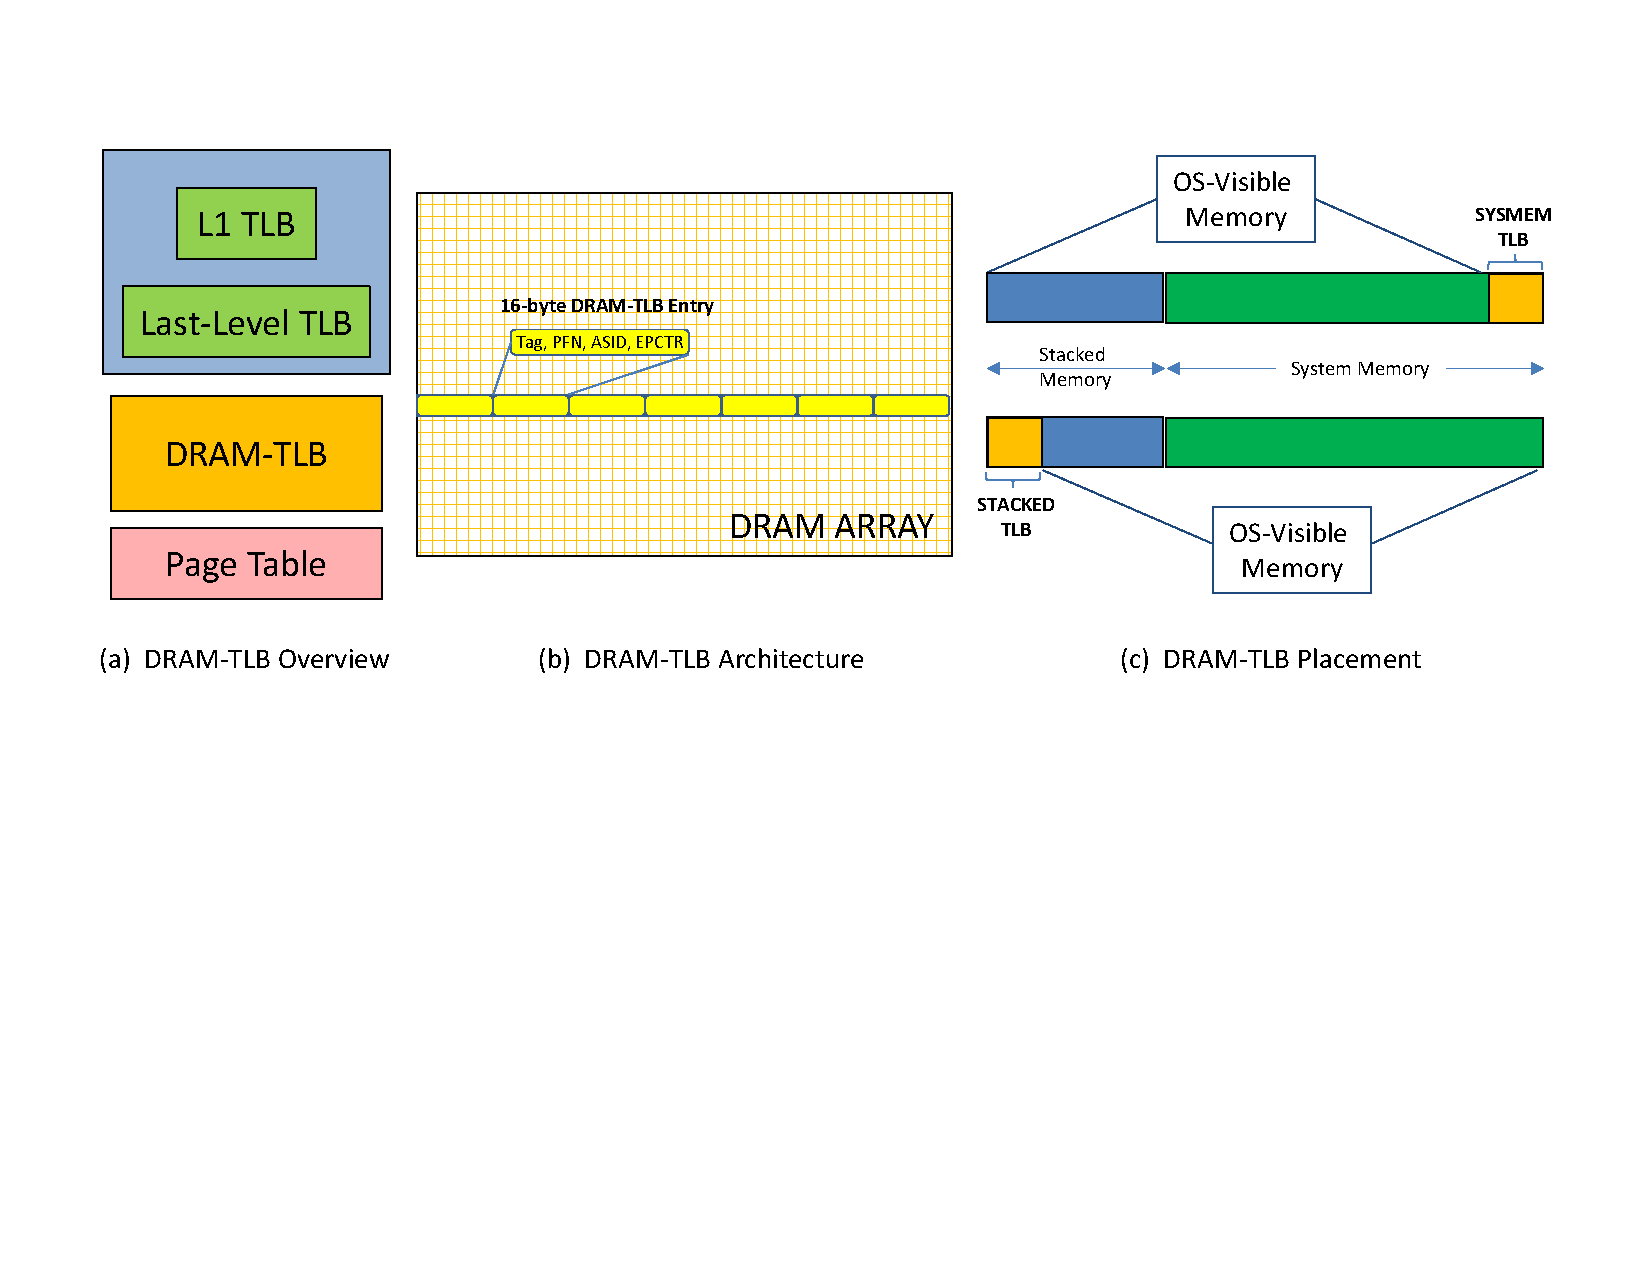
\psfig{file=FIGURES/stacked_tlb,width=\textwidth}}

  \caption{\small Improving TLB coverage by embedding TLBs in DRAM
    (DRAM-TLB). A DRAM-TLB architected using commodity DRAM is called
    SysMem-TLB and a DRAM-TLB architected with stacked DRAM is called
    Stacked-TLB. \normalsize}
  \label{fig:stacked_tlb} 
  \vspace{0.1 in}
\end{figure*}

\subsection{DRAM-TLB Architecture}

\noindent DRAM-TLBs can either be architected using stacked memory or
system memory. A DRAM-TLB architected using stacked memory is referred
to as a {\em Stacked-TLB} while a DRAM-TLB architected using system
memory is referred to as a {\em SysMem-TLB}. DRAM-TLBs are physically
placed in a large contiguous segment of memory and are entirely
hardware-managed. As such, DRAM-TLBs do not contribute to the
OS-visible memory space (see Figure~\ref{fig:stacked_tlb}(c)).

% illustrates, DRAM-TLBs and the OS-visible
% address space when the hybrid memory system is configured with a
% SysMem-TLB or a Stacked-TLB.

\subsubsection{DRAM-TLB Organization}

\noindent Like conventional on-chip SRAM TLBs, and the proposed UCAT
architecture, a DRAM-TLB entry maintains the TLB tag, physical
address, and meta data information such as valid bits, page permission
bits, address space identifier (ASID). To accommodate this
information, we propose 16 bytes of storage per DRAM-TLB entry.
Figure~\ref{fig:stacked_tlb} illustrates the layout of the DRAM-TLB in
the DRAM array. For example, a 2KB DRAM row buffer holds 128 DRAM-TLB
entries per row.

\newpage
\subsubsection{DRAM-TLB Lookups}

\noindent Unlike on-chip TLBs, all DRAM-TLB operations occur on the
DRAM data bus at the granularity of the DRAM interface. Thus, on an
LLT miss, if implemented as a stacked-TLB, the lookup fetches data at
the granularity of the stacked memory interface: 32-byte cacheline
(two TLB entries), and if implemented in system memory, the lookup
fetches data at the granularity of the DDR interface: 64-byte
cacheline (four TLB entries).

Reading multiple TLB entries enables architecting a set-associative
DRAM-TLB without incurring additional latency or
bandwidth~\cite{moin2012,loh2011}. 
%We explored the design space of
%set-associative and direct-mapped DRAM-TLBs. 
We evaluate both set-associative and direct-mapped
designs and observe similar performance among these design points with large DRAM-TLB sizes.
These results match the behavior of
existing work on large DRAM Caches where conflict misses tend to be
low~\cite{moin2012}. Thus, we architect a direct-mapped DRAM-TLB where
consecutive DRAM-TLB sets map to the same rowbuffer in memory (to
exploit DRAM row buffer locality). Adjacent DRAM-TLB entries fetched
are also inserted into the PWC for potential future hits.

We could further take advantage of reading multiple TLB entries with a
single read operation. Retrieving the co-located DRAM-TLB entries on a
DRAM-TLB read naturally enables prefetching of neighboring address
translations. For example, prefetched entries can be stored in an
on-chip TLB prefetch buffer. This approach is similar to caching
co-located page table entries in the PWCs on a conventional page table
walk. We leave the evaluation of such designs to future work.


% Similar to page walk caches, we also provision an 8-entry
% DRAM-TLB-Cache (DTLBcache) that stores recent lines retrieved from the
% DRAM-TLB. In doing so, the DTLBcache exploits spatial locality in LLT
% misses.

\subsubsection{DRAM-TLB Insertions and Updates}

\noindent The DRAM-TLB must be updated on misses, shootdowns, and page
permission changes. We propose to modify the TLB-entry directly in
DRAM on updates. To ensure that updating a single DRAM-TLB-entry does
not corrupt the contents of co-located DRAM-TLB entries, we leverage
existing DRAM interfaces that allow partial writes (e.g. byte-level
writes) to memory without the power and bandwidth overhead of a full
read-modify-write operation~\cite{hbm-spec}.

% Note that a direct-mapped DRAM-TLB architecture also helps avoid a
% read-modify-write operation. If the DRAM-TLB were set-associative, a
% read is necessary to determine which DRAM-TLB way .

% If the DRAM-TLB entry exists in the DTLBcache, the corresponding entry
% is directly updated in the DTLBcache. However, if the entry does not
% exist in the DTLBcache,




% \begin{figure}[htb] 
% \vspace{-0. in}
% \centering
% 	\centerline{\psfig{file=GRAPHS/stackedDRAMTLB_cachelat,angle=-90,width=\columnwidth}}
% 
% \caption{\small This figure compares the average LLC miss latency of
% 	DRAM-TLB and Stacked-TLB relative to the baseline system. \normalsize}
% \label{fig:cachelat_DRAMTLB} 
% \vspace{-0. in}
% \end{figure}

\subsubsection{DRAM-TLB Implementation}

% If the request can be serviced from the first-level page table, the
% MMU follows the baseline address translation policy and fetches the
% translation from the first-level page table. This is because
% retreiving the first-level page table entry and a DRAM-TLB lookup both
% require a single memory access.

% If the MMU is required to access more than one level of the page
% table, we propose that the

\noindent Since the DRAM-TLB is stored in physical memory, the
physical address for the DRAM-TLB entry must be computed. We propose
an 8-byte register in the Memory Management Unit (MMU) to store the
base address $BaseAddr$ for the DRAM-TLB. Given the DRAM-TLB set index
{\em SI}, DRAM-TLB associativity $A$, and DRAM-TLB entry size $s$ (16
bytes in our case), the MMU computes the physical address for the
DRAM-TLB entry using combinational logic:

\begin{equation}
  \begin{array}{rl}
    \text{PhysAddr} = BaseAddr + SI * A * s
  \end{array}
\end{equation}

\noindent Once the DRAM-TLB entry is retrieved from memory, the MMU
compares the tag to determine hit or miss. On a DRAM-TLB hit, the
missing translation is returned to the processor. However, on a
DRAM-TLB miss, the MMU walks the application page table to determine
the virtual to physical translation. This translation is returned to
the processor and also inserted into the DRAM-TLB.

\subsubsection{DRAM-TLB Example}

\noindent Assume a 1M-entry direct-mapped DRAM-TLB (with 4KB pages)
starting at memory location {\em BaseAddr=0}. An LLT miss for virtual
page 0xff2212345000 requires fetching the 16-byte DRAM-TLB entry at
set index 0x12345. With $A=1$ and $s=16$, the physical memory location
for this DRAM-TLB entry is 0x123450 (i.e. 0 + 0x12345 * 1 * 16). The
MMU compares the missing tag (0xff22) with the DRAM-TLB entry to
determine DRAM-TLB hit or miss.

% \ee{if we start running out of space this sort of thing is probably a
% bit redundant}

\begin{figure}[tp] 
  \vspace{-0.in} \centering
  \centerline{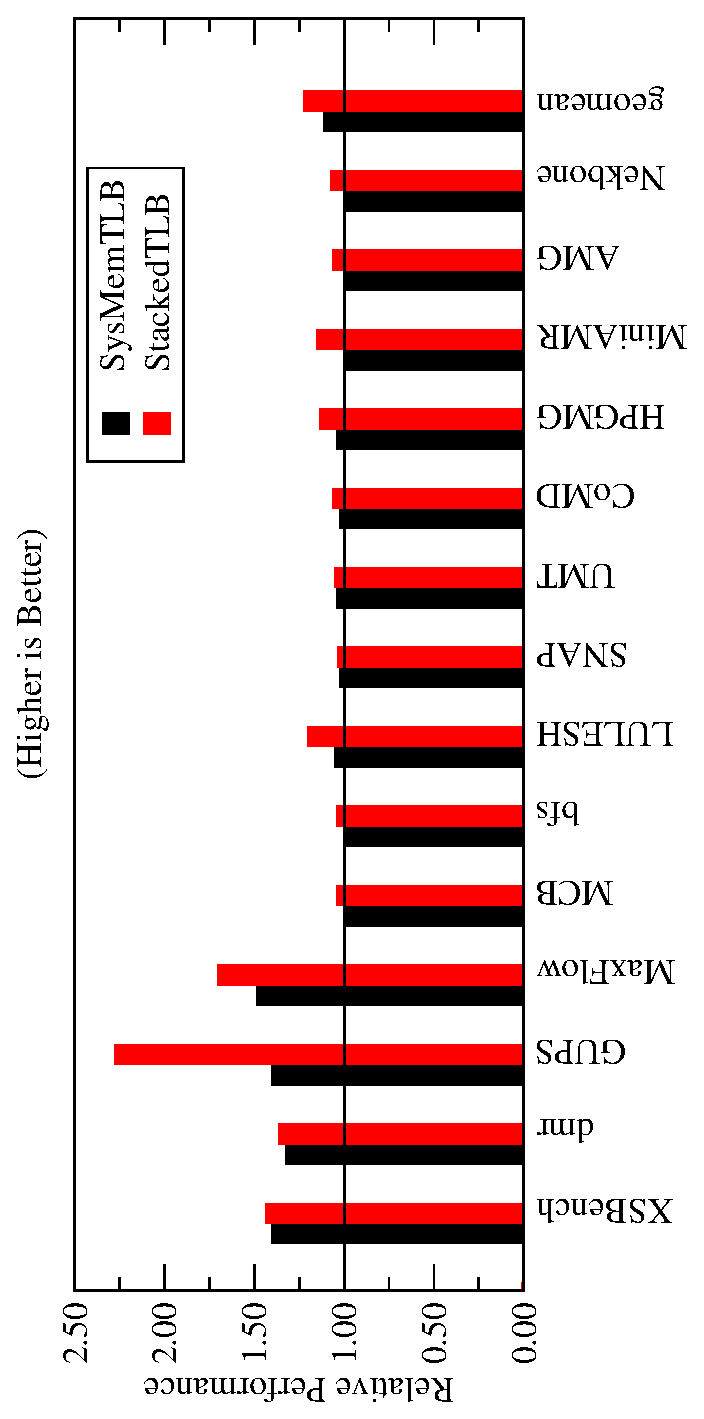
\psfig{file=GRAPHS/DRAMTLB_perf,angle=-90,width=\columnwidth}}

  \caption{\small Performance of DRAM-TLBs. \normalsize}
  \label{fig:perf_DRAMTLB} 
  \vspace{0.2 in}
\end{figure}

\begin{figure}[tp] 
  \vspace{0.in} \centering
  \centerline{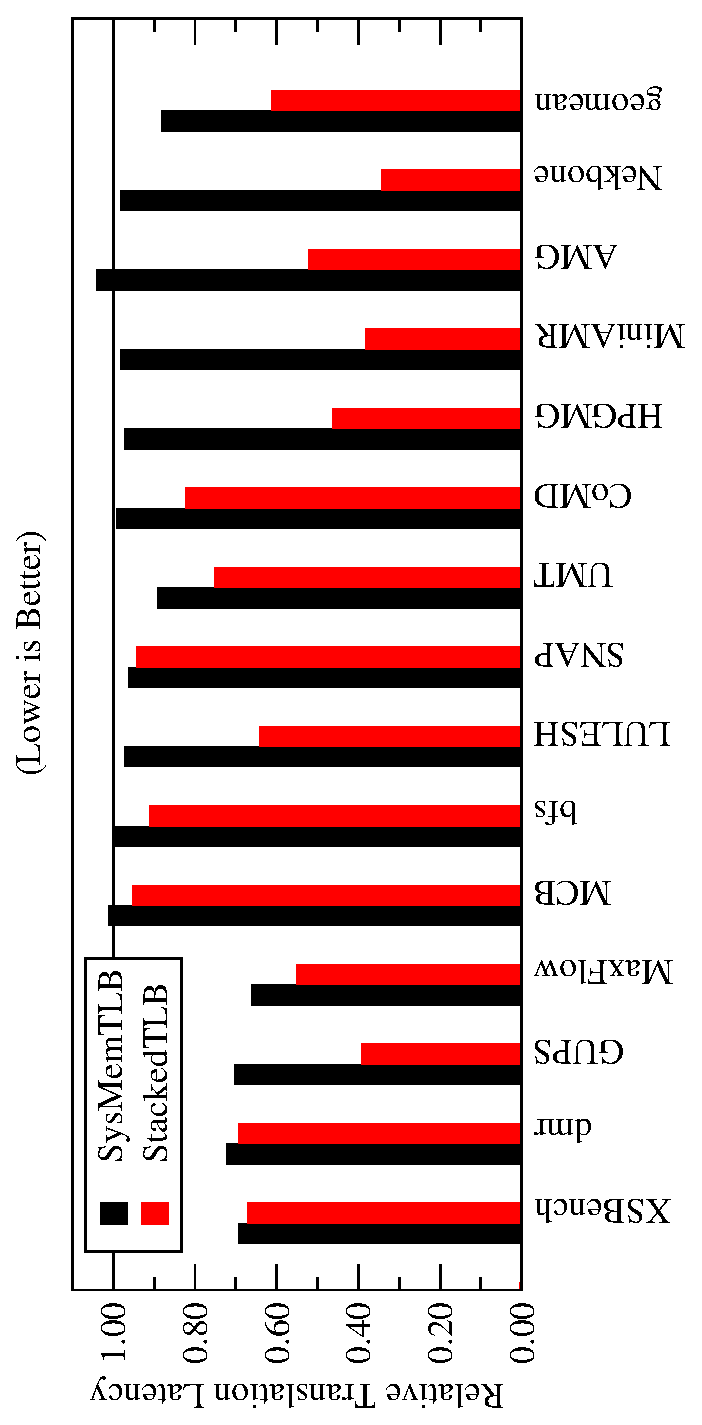
\psfig{file=GRAPHS/DRAMTLB_tlblat,angle=-90,width=\columnwidth}}

  \caption{\small Relative Translation Latency.\normalsize}
  \label{fig:tlblat_DRAMTLB} 
%  \vspace{0.2 in}
\end{figure}

% \begin{figure}[b] 
%   \vspace{0.2in} \centering
%   \centerline{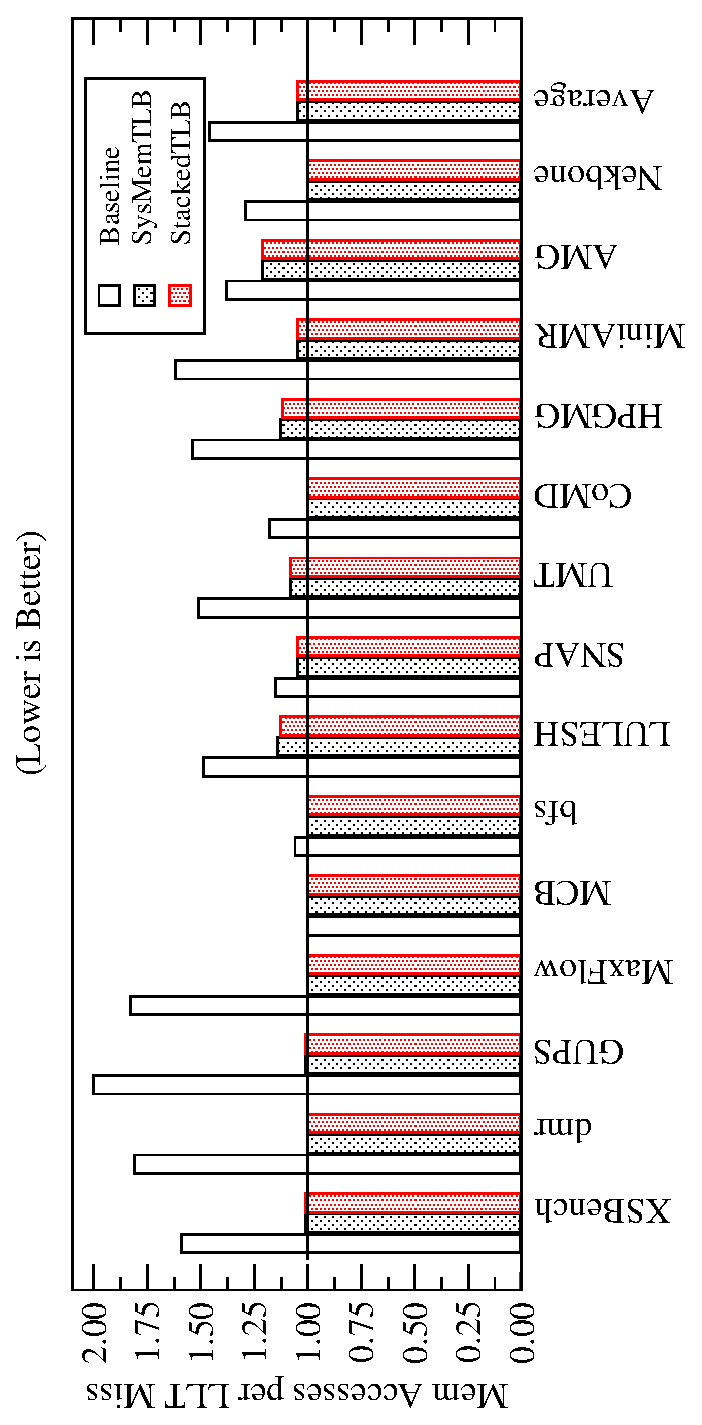
\psfig{file=GRAPHS/DRAMTLB_pteaccess,angle=-90,width=\columnwidth}}
% 
%   \caption{\small Memory Accesses on an LLT miss.\normalsize}
%  \label{fig:memaccess_DRAMTLB} 
%   \vspace{0.0 in}
% \end{figure}

\subsection{DRAM-TLB Performance}

% For our evaluation purposes, we do not exploit the prefetching
% benefits from fetching multiple TLB entries with a single DRAM read
% operation.

% \subsubsection{Steady State Performance Behavior}

% Since our application
% have memory footprint less than 32GB, both DRAM-TLB configurations
% incur only compulsory misses and behave like a {\em perfect} DRAM-TLB
% in steady state.

% illustrates the workloads on the x-axis and the performance relative
% to our baseline system on the y-axis. The figure

\noindent We evaluate SysMem-TLB and Stacked-TLB performance assuming
an 8-million entry DRAM TLB (32GB TLB coverage with 4KB pages).
Figure~\ref{fig:perf_DRAMTLB} shows that DRAM-TLBs improve performance
relative to the baseline system across all TLB-sensitive workloads. On
average, SysMem-TLB improves performance by 11\% while Stacked-TLB
improves performance by 22\%. 

Figure~\ref{fig:tlblat_DRAMTLB} shows that SysMem-TLBs reduce address
translation latency by 12\% while Stacked-TLBs reduce address
translation latency by 40\%. In general, Stacked-TLBs perform better
than SysMem-TLBs because they are architected with stacked memory, a
technology that provides lower memory queuing delay due to the high
memory bandwidth. Our studies show that the loaded stacked memory
latency tends to be 8-15x lower than system memory access latency.

DRAM-TLBs decrease address translation latency by reducing the number
of memory accesses on an LLT miss. Figure~\ref{fig:memaccess_DRAMTLB}
shows that the baseline system incurs 1.5 memory accesses per LLT miss
(up to 2) on average. On the other hand, both SysMem-TLB and
Stacked-TLB incur only 1.05 memory access per LLT miss (max of 1.21)
on average. By reducing the number of memory acceses, DRAM-TLBs boost
performance of TLB-sensitive workloads like $GUPS$ by 2.2$x$ and
$MaxFlow$ by 70\%. Furthermore, workloads like $XSBench$, $dmr$,
$LULESH$, and $MiniAMR$ experience more than 15\% performance gain.
These results show that DRAM-TLBs successfully decrease LLT miss
latency by reducing the number of memory accesses on an LLT miss.

% % \subsubsection{Non-Steady State Performance Behavior}
% % 
% % \noindent Under steady state conditions, SysMem-TLBs are competitive
% % with Stacked-TLB despite being architected using low bandwidth
% % commodity DRAM. However, in practice workloads tend to go through
% % phases of execution where misses occur in the DRAM-TLB. As such, we
% % now study how SysMem-TLBs and Stacked-TLBs behave when they experience
% % TLB misses.
% % 
% % \begin{figure}[t] 
% %   \vspace{-0. in}
% %   \centering
% %   \centerline{\psfig{file=GRAPHS/stackedDRAMTLB_hitrate_sens,angle=-90,width=\columnwidth}}
% % 
% %   \caption{\small Sensitivity to DRAM-TLB hit-rate. \normalsize}
% % 
% %   \label{fig:hitrate_DRAMTLB} 
% %   \vspace{-0. in}
% % \end{figure}
% % 
% % The overhead of a DRAM-TLB miss is the wasted bandwidth to consult the
% % DRAM-TLB and the bandwidth to insert the missing entry into the
% % DRAM-TLB. In general, these operations consume precious DRAM
% % bandwidth. When bandwidth is scarce, both these operations can degrade
% % performance significantly since they do not contribute towards useful
% % work. To understand this phenomenon,
% % Figure~\ref{fig:hitrate_DRAMTLB} illustrates the performance
% % behavior of SysMem-TLBs and Stacked-TLBs as a function of
% % hit-rate\footnote{A statistical model that samples a random number
% % generator is used to achieve the desired DRAM-TLB hit rate.}. The
% % x-axis shows the TLB hit rate while the y-axis shows the performance
% % relative to the baseline system averaged across all workloads.
% % 
% % In steady state (i.e. when the TLB hit rate is a 100\%) both
% % Stacked-TLB and SysMem-TLB perform well. However, when the hit-rate
% % reduces, DRAM-TLB lookup and DRAM-TLB fill operations start consuming
% % precious DRAM bandwidth. This additional bandwidth quickly degrades
% % SysMem-TLB performance. For example, at 80\% hit rate, SysMem-TLB
% % performance plunges from 38\% performance improvement to a mere 8\%
% % performance improvement. Continuing to follow the hit-rate curve,
% % SysMem-TLBs degrade performance at DRAM-TLB hit-rates below 70\%.
% % These results show that SysMem-TLBs are useful only if they can
% % provide near-optimal hit-rate. Unfortunately ensuring a 100\% hit-rate
% % is impossible without future knowledge.
% % 
% % Stacked-TLBs are less sensitive to degradation in hit-rate. An 80\%
% % Stacked-TLB hit-rate retains performance improvement (34\% vs 42\%).
% % Following the hit-rate curve, Stacked-TLBs degrade performance only
% % when the hit-rate drops below 30\% (which is unlikely). Consequently,
% % this suggests that Stacked-TLBs are more suitable alternative to
% % SysMem-TLBs. Hereon, we only report performance results for
% % Stacked-TLBs.

% <------------GRAVEYARD
% Both DRAM-TLB and Stacked-TLB improve performance because they reduce
% the address translation bandwidth and address translation latency. In
% doing so, the LLT miss latency reduces by (see ).

% Furthermore, since Stacked-TLBs handle changes in hit-rate gracefully,
% we report performance results for workloads in steady state.

% This suggests that the bandwidth capability of stacked memory enables
% Stacked-TLBs as a viable hardware structure to increase the TLB
% hierarchy.

% Unfortunately, the first order performance bottleneck of DRAM-TLB
% misses is bandwidth. If the DRAM-TLB lookup misses, that is wasted
% bandwidth. Inserting a missing translation into the DRAM-TLB requires
% bandwidth.

% Consequently such requests consume precious system memory bandwidth.
% Furthermore, to DRAM-TLBs

% If DRAM-TLBs can constantly provide hits, they reduce the 1.75 memory
% accesses per LLT miss our workloads observe to a single memory access.
% However, DRAM-TLBs can suffer from misses too. Especially when the
% application footprint exceeds the coverage of the DRAM-TLB. This
% problem can be addressed by simply sizing the DRAM-TLB to cover the
% largest possible application memory footprint. In our experience, the
% majority of DRAM-TLB misses are compulsory misses. Once the workload
% reaches steady state, a DRAM-TLB effectively behaves like a {\em
% perfect} TLB.

% If the workloads frequently miss in the DRAM-TLB, both the latency and
% required bandwidth for address translation increases. This is because
% a DRAM-TLB miss incurs two additional memory accesses: one for missing
% in the DRAM-TLB and the other for inserting the missing DRAM-TLB.


% Note, however that the DRAM-TLB lookup is on the critical path while
% the DRAM-TLB fill can be done in the background. Thus, the memory
% bandwidth penalty of a DRAM-TLB miss is two requests, but the latency
% penalty is one memory access.

% Therefore, the total cost
% of a DRAM-TLB miss is the cost of one memory access serialization latency plus
% any queuing delays due to the DRAM-TLB fill.

% To quantify the desired behavior of DRAM-TLBs, both from miss traffic
% and miss latency perspective, 

% Figure~\ref{fig:hitrate_DRAMTLB} illustrates the required
% DRAM-TLB hit rate to equalize the average address translation traffic
% and the average address translation latency (assuming DRAM-TLB fills
% do not significantly impact memory access latency) respectively. The
% x-axis illustrates the average number of page table memory accesses
% per LLT miss while the y-axis illustrates the required DRAM-TLB hit
% rate.

% Clearly, if the average number of page table accesses per LLT miss is
% one, we would require a 100\% DRAM-TLB hit rate. As described earlier
% in the paper, this would normally occur when the MMU always hits in
% the second-level page table cache. In such situations, the MMU can
% just bypass the DRAM-TLB lookup altogether and just fetch the
% translations directly from the page table.
% 
% However, the majority of our applications require more than one page
% table access per LLT miss (ranging between 1.40 and 2.25). These page
% table access rates require a DRAM-TLB hit-rate ranging between 40\%
% and 80\%. Achieving these hit rates is well within the range of
% DRAM-TLBs because their relative storage overhead is negligible.
% However, in pathological situations where the DRAM-TLB hit-rate is
% well below the desired break-even hit rate (e.g. streaming workload),
% the MMU can dynamically bypass the DRAM-TLB state machine altogether.


% \begin{figure}[t] 
% \vspace{-0. in}
% \centering
% 	\centerline{\psfig{file=GRAPHS/stackedDRAMTLB_break_even,angle=-90,width=\columnwidth}}
% 
% \caption{\small This figure illustrates a sensitivity study for the
%   required DRAM-TLB hit rate for different pagetable requests per LLT miss. \normalsize}
% \label{fig:hitrate_DRAMTLB} 
% \vspace{-0. in}
% \end{figure}
%------------------> GRAVEYARD
\newpage
\subsection{DRAM-TLB Design Overhead}

\noindent Figure~\ref{fig:mmu_state} shows simple modifications to the
Memory Management Unit (MMU) state machine to support DRAM-TLBs. On an
LLT miss, the MMU first consults the PWCs to retrieve the translation.
If the request misses in the PWCs, the MMU consults the DRAM-TLB. If
the request misses in the DRAM-TLB, the MMU walks the page table.
Thus, we simply introduce a new state in the MMU state machine for the
DRAM-TLB lookup before walking the page table.

The in-memory storage overhead for DRAM-TLBs depends on the desired
TLB coverage. For example, achieving full system memory (256GB in our
baseline) coverage with 4KB, 64KB, and 2MB pages requires 1GB, 64MB,
and 2MB of storage overhead respectively (assuming 16-byte DRAM-TLB
entries). In general, this storage overhead is impractical for on-chip
SRAM TLBs. However, these sizes are an insignificant fraction of
emerging multi-gigabyte DRAM systems. For example, the aforementioned
storage overheads correspond to 6\% (4KB pages), 0.4\% (64KB pages),
and 0.01\% (2MB pages) storage overhead for a 16GB stacked memory
system. Consequently, DRAM-TLBs improve TLB coverage using small pages
with minimal storage overhead and require no significant changes to
the existing address translation architecture. 

Like UCAT, DRAM-TLBs also require efficient support for handling TLB
shootdown and TLB flush requests. We discuss these design issues in
Section~\ref{sec:implications}.

\begin{figure}[tp] 
  \vspace{0.2in} \centering
  \centerline{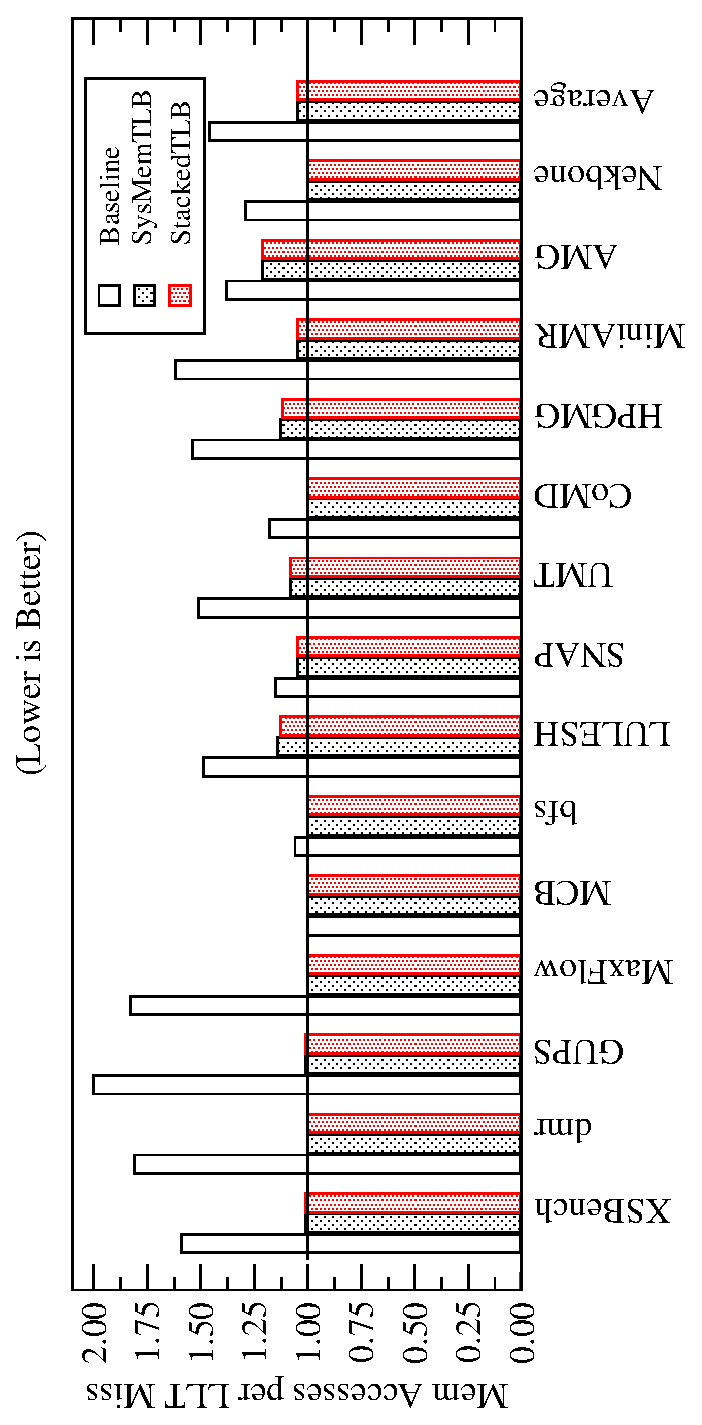
\psfig{file=GRAPHS/DRAMTLB_pteaccess,angle=-90,width=\columnwidth}}

  \caption{\small Memory Accesses on an LLT miss.\normalsize}
 \label{fig:memaccess_DRAMTLB} 
  \vspace{0.0 in}
\end{figure}


\begin{figure}[b] 
  \vspace{-0. in} \centering
  \centerline{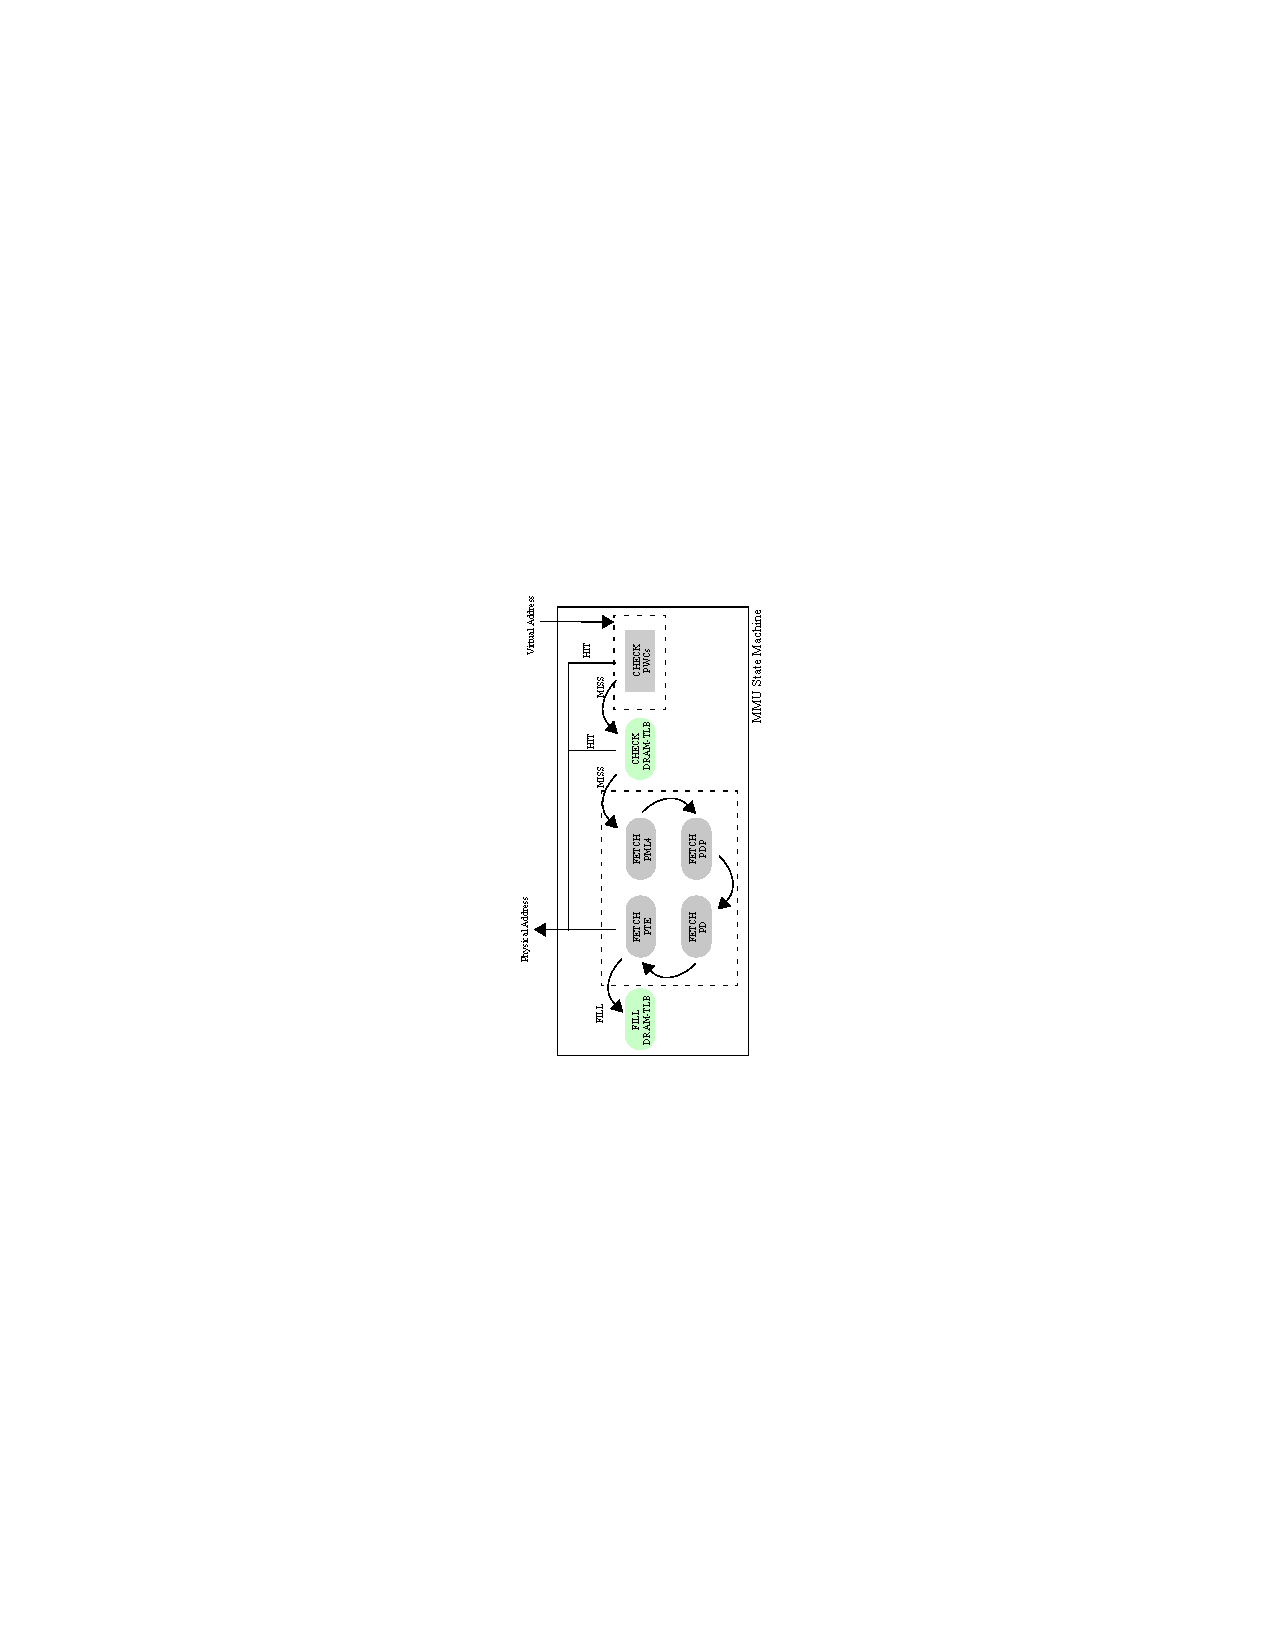
\psfig{file=FIGURES/mmu_state,angle=-90,width=\columnwidth}}

  \caption{\small MMU extensions to support DRAM-TLBs.
    \normalsize}
  \label{fig:mmu_state} 
  \vspace{-0 in}
\end{figure}



% \subsection{DRAM-TLB Summary}
% 
% \noindent DRAM-TLB is a flexible, scalable, and low overhead mechanism
% that can provide arbitrary TLB coverage. DRAM-TLB serves as the next
% shared level in the on-chip TLB hierarchy and can reduce memory
% bandwidth requirements for address translation to a single memory
% access and can improve performance by 50\% on average (up to 2X).

% DRAM-TLBs provide an opportunity to increase the coverage of existing
% on-chip TLB hierarchies. Since, DRAM-TLBs can potentially provide
% address translations using in a single memory access, they provide an
% alternative low latency, low bandwidth solution to walking the page
% table on an LLT miss.


